\documentclass[12pt]{article}

\usepackage{templates/sbc-template}

\usepackage{graphicx,url}
\usepackage{color}

\usepackage[brazil]{babel}
\usepackage[utf8]{inputenc}


\sloppy

\title{Identificação e classificação de comentários tóxicos utilizando processamento de linguagens naturais e técnicas de aprendizagem profunda}

\author{
    Miguel Angelo Cece de Castro Neto\inst{1},
    Paulo Alves dos Santos Junior\inst{1}\\
    Alceu de Souza Britto Junior\inst{2}
}


\address{
    Departamento de Informática -- Universidade Estadual de Ponta Grossa (UEPG)\\
    Avenida General Carlos Cavalcanti, 4748\\
    CEP 84030-900 – Ponta Grossa, PR – Brasil
    \nextinstitute
    Programa de Pós-Graduação em Informática (PPGIa) – Pontifícia Universidade\\
    Católica do Paraná (PUCPR)\\
    Rua Imaculada Conceição, 1155\\
    CEP 80215-901 – Curitiba, PR – Brasil
    \email{miguelceccineto@gmail.com, contato@pauloalvesjr.com,
     alceu@ppgia.pucpr.br}
}

\begin{document}

\maketitle

\begin{abstract}
  The article addresses the problem of multiclass sentiment analysis at the sentence level. Recurrent neural networks and their demonstrations have demonstrated successful modeling of feeling classifiers and last generation in language modeling with the same demonstration demonstrating efficiency and performance in various tasks. The datasheet of the learned paper transfer, larger database, has proven effective in small databases. In the paper we propose the use of combinations of architecture together with a combination of convolutional techniques.
\end{abstract}

\begin{resumo}
  Este artigo aborda o problema da análise de sentimentos multiclasse no nível de sentença. Redes neurais recorrentes e suas variações demonstraram sucesso na modelagem de classificadores de sentimentos e recentemente a modelagem de linguagens através dessa arquitetura demonstrou-se eficaz atingindo o estado da arte em várias tarefas. O uso da técnica de transferência de aprendizado, proveniente de banco de dados maiores, se demonstrou eficiente em banco de dados pequenos. Nesse trabalho propomos o uso destas variações arquitetura em conjunto com a combinação de técnicas convolucionais.
\end{resumo}


\section{Introdução} \label{sec:introducao}

Discutir assuntos na internet pode ser difícil. Ameaças, ofensas pessoais, e assédio, podem criar um ambiente tóxico dentro de fóruns e redes sociais, e até afastar usuários. As plataformas lutam para combater efetivamente discussões tóxicas e limitar ou desligar usuários com essas práticas, porém essa é uma tarefa de difícil automação exigindo milhares de sentenças rotuladas e métodos capazes de analisar de maneira eficaz o contexto e significado.

Recentemente, em resposta ao crescimento do uso de redes sociais, comentários são publicados massivamente. Como a escrita compõe grande parte de todos os dados gerados pela humanidade, que até então, apenas serviam para consultas, hoje servem como base de dados para o desenvolvimento de sistemas de processamento de linguagens naturais. Aplicando técnicas de aprendizagem profunda podemos automatizar processos, análises e classificação de textos com uma boa taxa de acerto, comparado à métodos bayesianos, por exemplo.

No problema a ser discutido nesse artigo, com base de dados referente a comentários tóxicos, temos basicamente a análise de sentimentos conforme as classes rotuladas, sendo utilizada para representar em quais classes de toxicidade determinada sentença pertence. Formalmente, o objetivo da análise de sentimentos nesse trabalho é extrair a seguinte sêxtupla:

\[
(a\lambda1, a\lambda2, a\lambda3, a\lambda4, a\lambda5, a\lambda6)
\]

Onde $a \lambda i$ se refere a probabilidade de cada classe, que respectivamente representam: Tóxico; Muito Tóxico; Obsceno; Ameaça; Insulto; Ódio de Identidade.

A análise de sentimentos é determinada comumente de maneira binária (positiva e negativa), porém abordagens multiclasse também são possíveis. Em uma abordagem multiclasse determinado comentário pode possuir diversos rótulos simultaneamente. Para definir a ativação de determinada classe, é definido um limiar. Tal limiar só é válido devido a função de ativação utilizada como saída na rede.

A utilização de redes neurais artificiais voltou a popularizar-se no reconhecimento de padrões em imagens devido a evolução de hardware, tais métodos de aprendizagem de máquina combinados ao processamento de linguagens naturais, permitem a avaliação automática de padrões e extração de conhecimento de bases de texto. A identificação de comentários ofensivos em textos é um derivado do caso geral de análise de sentimentos, na era da internet, identificar e classificar sentenças permite tomada de decisões e maior controle e filtragem de conteúdo. 

Esse trabalho tem como principal interesse, o estudo e experimento de técnicas de aprendizagem profunda (\textit{deep learning}) aplicada à área de processamento de linguagens naturais. Abordagens de aprendizagem de máquina tradicionais necessitam de intervenção humana para definição de características, existe a possibilidade de delegar tal tarefa à algoritmos simples de extração de características línguisticas ou sintáticas disponíveis na literatura, como utilizando contagem \cite{DBLP:journals/corr/abs-1805-04871}, ou processamento esparso \cite{ramos2003using}. A tarefa realizada utilizando métodos clássicos, por fim utilizam algum método superficial de aprendizado, como por exemplo, máquinas de vetores de suporte \cite{DBLP:journals/ml/CortesV95}, naive bayes e máquinas de vetores de suport naive bayes  \cite{wang:2012}.

Embora os métodos descritos anteriormente já tenham sido validados, o foco desse trabalho é utilizar um método automátizado de extração de características que seja eficaz. Para a análise de sentimentos em comentários e classificação de toxicidade, utilizaremos utilizaremos redes neurais recorrentes em conjunto com estruturas celulares específicas, como células recorrentes bloqueadas (\textit{gated recurrent units}) \cite{DBLP:journals/corr/PascanuGCB13} e células de longa memória de curto termo (\textit{long-short term memory}) \cite{sep:97}. Abordaremos técnicas de transferência de aprendizado e aplicação de módulos convolucionais \cite{lecun:98}.
A estrutura recorrente é uma variação da rede neural clássica para aceitar entradas com tamanhos e saídas arbitrários, possuindo também registro de contexto em relação a posição do elemento em seu conjunto de entrada. Redes recorrentes comuns não são efetivas devido a problemas de esquecimento de aprendizado ou pouca capacidade de aprendizado devido a limitação imposta pela quantidade de parâmetros. Para resolver essa situação existem diferentes células que podem ser incorporadas nas arquiteturas, como por exemplo células recorrentes bloqueadas (\textit{gated recurrent units}) e células de longa memória de curto termo (\textit{long-short term memory}).

As redes neurais recorrentes possuem como característica a capacidade de trabalhar com entradas e saídas de tamanhos arbitrários, sendo uma ótima arquitetura para solução de problemas de múltiplas sentenças. É apenas necessário o pré-processamento de cada elemento, com o objetivo de remoção de ruídos e conversão para tensores numéricos \cite{karpathy:2015}.

A adição de convoluções, também podem ser utilizadas, para melhorar a detecção de padrões nas saídas de redes recorrentes. As redes convolucionais normalmente são utilizadas para extração de características em imagens \cite{lecun:98} ou quando as dimensões estão extremamente relacionadas. No caso imagens, são utilizadas convoluções de duas dimensões, no caso de vídeo ou objetos tridimensionais, três dimensões. Nesse artigo será avaliado o desempenho de convoluções de uma dimensão buscando o relacionamento dessas saídas.

Nesse trabalho as arquiteturas utilizadas aspiram utilizar os diversos conceitos disponíveis em busca de uma solução melhor que o aprendizado de máquina clássico e conceitos individuais. Na seção 2 é descrito brevemente trabalhos relacionados na área, tanto em aprendizado de máquina clássico, quanto aprendizado de máquina profundo. Na seção 3 revisaremos os principais conceitos para o entendimento da seção 4, que se refere as arquiteturas utilizadas nesse artigo. Na seção 5 temos a análise e comparação de todos os modelos treinados, já na seção 6 nossas considerações finais e trabalhos futuros.

\section{Trabalho Relacionado} \label{sec:relacionado}

A análise de sentimentos está sob grande aprimoramento devido a aplicação de redes recorrentes \cite{karpathy:2015}, redes convolucionais \cite{lecun:98} e transferência de aprendizado \cite{DBLP:journals/corr/abs-1801-06146}. Esses casos descritos anteriormente se referem ao estado da arte dessa atividade.

Métodos clássicos de aprendizagem de máquina aplicados a análise e classificação de sentimento, como por exemplo \textit{Suport Vector Machines} \cite{DBLP:journals/ml/CortesV95}, apresentam resultados inferiores ao estado da arte. Essa abordagem necessita que as características sejam extraídas de maneira não automátizada, com ajuda de análise humanada, ou utilizando segmentações pouco eficientes, como por exemplo contagem de palavras e transformações esparsas.

O principal problema do método superficial citado acima, é que ele não é capaz de identificar o contexto de palavras, não sendo uma opção robusta para classificação.

Redes recorrentes e suas variações são aplicadas utilizando comumente matrizes que definem significado próximos ao real para cada palavra, como por exemplo \textit{Word2Vec} \cite{DBLP:journals/corr/abs-1301-3781} ou \textit{GloVe} \cite{pennington2014glove}. Tais métodos provem contexto utilizando palavras próximas para modelas matrizes e consequentemente contexto para redes recorrentes.

Transferência de aprendizado é uma técnica onde um modelo já treinado é reajustado para detectar padrões diferentes dos iniciais. Geralmente usado quando a base de dados disponível é menor do que a usada no modelo já treinado. Trabalhos recentes propõem a utilização de modelos de linguagem universais, que sofrerão afinação (fine tuning) para atender uma tarefa específica \cite{DBLP:journals/corr/abs-1801-06146} com a possibilidade de utilização de dados não supervisionados para gerar um aumento de performance (Radford et al. 2018). A utilização de dados não rotulados permite reduzir drasticamente a necessidade de exemplos rotulados. O estado da arte da maioria das tarefas na área de linguagens naturais está relacionado ao uso de transferência de aprendizado e aprendizado não supervisionado, que é um dos maiores desafios atualmente.

\section{Redes Neurais} \label{sec:revisao}
\subsection{Redes Artificiais Profundas (\textit{deep feedforward networks})}

Redes \textit{feedforward} profundas, também chamadas de redes neurais feedforward, ou perceptrons multicamadas (\textit{multilayer perceptrons}), são essenciais nos modelos de aprendizagem profunda. O objetivo de uma rede feedforward é aproximar uma função $f$. Por exemplo, para um classificador, $y = f ∗ (x)$ mapeia uma entrada $x$ para uma categoria $y$. Uma rede feedforward define um mapeamento $y = f (x; θ)$ e aprende o valor dos parâmetros $θ$ que resultam na melhor aproximação da função.

Esses modelos são chamados \textit{feedforward} porque a informação flui através da função que está sendo avaliada de $x$, através dos cálculos intermediários usados ​​para definir $f$ e, finalmente, para a saída $y$. Não há conexões de retroalimentação nas quais as saídas do modelo são realimentadas. Quando redes neurais \textit{feedforward} são estendidas para incluir conexões de retroalimentação, elas são chamadas de redes neurais recorrentes.

As redes \texit{feedforward} são de extrema importância para os profissionais de aprendizado de máquina. Eles formam a base de muitas aplicações comerciais importantes. Por exemplo, as redes convolucionais usadas para reconhecimento de objetos em imagens são um tipo especializado de rede \textit{feedforward}. As redes da \textit{feedforward} são um trampolim conceitual no caminho para redes recorrentes, que potencializam muitas aplicações de linguagem natural. \cite{Goodfellow-et-al-2016}.

\subsection{Redes Neurais Recorrentes}

Redes recorrentes possuem o mesmo conceito básico de redes neurais artificiais, com o objetivo de otimizar parâmetros para retornar uma saída coerente em relação a entrada e ao problema. O que faz as redes recorrentes serem especiais, é o fato de elas não possuirem a restrição de tamanho fixo de entrada ou saída \cite{karpathy:2015}.

O conjunto de dados utilizados nesse artigo se adequa a arquitetura muitos para muitos, onde a entrada são as sequencias vetorizadas e tratadas através de \textit{word embeddings}) e a saída é um vetor de probabilidades das classes.

O modelo muitos para muitos nesse conjunto de dados, possuirá a entrada onde cada bloco terá o número de \textit{minibatches} de matrizes de \textit{word embeddings} para cada palavra.

A saída se comportará como representado anteriormente, sendo a sêxtupla:

\[
(a\lambda1, a\lambda2, a\lambda3, a\lambda4, a\lambda5, a\lambda6)
\]

Onde $a \lambda i$ se refere a probabilidade de cada classe, que respectivamente representam: Tóxico; Muito Tóxico; Obsceno; Ameaça; Insulto; Ódio de Identidade.

A imagem a seguir demonstra alguns casos de redes recorrentes possíveis:

\begin{figure}[!htb]
\centering
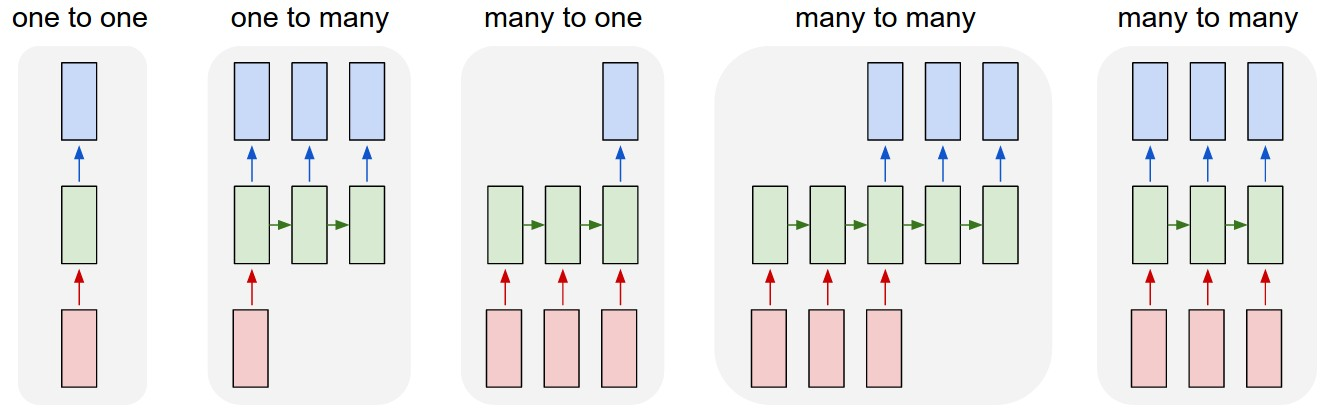
\includegraphics[width=1\textwidth]{images/rnn-effectiveness-examples.jpeg}
\caption{
    Possibilidades de entrada de saída em redes reccorentes. \cite{karpathy:2015}
}
\label{fig:sigmoid}
\end{figure}

\subsection{Funções de ativação}

Funções de ativação não lineares, dão capacidades não lineares para redes neurais \cite{lecun:98}. As funções de ativação nos permitem ir além de problemas linearmente separáveis. Caso essas funções não sejam adicionadas, o modelo apenas terá a capacidade de resolver problemas simples, sendo que todas as camadas formarão apenas um modelo linear.

É possível visualizar de maneira trivial na representação abaixo:

\begin{equation}
    z_1(z_0; w, b) = z_0^T * w_1 + b
\end{equation}

\begin{equation}
    z_2(z_1; w, b) = z_1^T * w_2 + b
\end{equation}

\begin{equation}
    z_2(z_1; w, b) = (z_0^T * w_1 + b)^T * w_2 + b
\end{equation}

A função (3), mesmo após a progressão através das camadas, continua sendo um modelo linear.

\subsubsection{ReLU - \textit{Rectified Linear Activation Function}}

Dada pela fórmula:

\begin{equation}
    ReLU(Z) = max(0, Z)
\end{equation}

A imagem abaixo descreve expressão da ReLU em um intervalo de 5 a –5.

\begin{figure}[!htb]
\centering
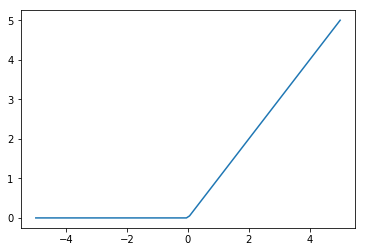
\includegraphics[width=.5\textwidth]{images/relu.png}
\caption{Unidade Linear Retificada}
\label{fig:relu}
\end{figure}

É a função de otimização padrão recomendada para uso na maioria das redes neurais. Aplicando essa função na saída de uma transformação linear produz uma transformação não linear \cite{nair2010rectified}.

A função permanece muito próxima de ser linear, contudo, no sentido de que é uma função linear por partes com duas peças lineares. Como as unidades lineares retificadas são quase lineares, elas preservam as propriedades que tornam os modelos lineares fáceis de otimizar com métodos baseados em gradiente. Eles também preservam muitas das propriedades que fazem modelos lineares generalizarem sistemas a partir de componentes mínimos \cite{Goodfellow-et-al-2016}.


\subsubsection{Sigmoide}

A função sigmoide é dada pela formula:

\begin{equation}
    \sigma(Z) = 1/(1+e^{-Z})
\end{equation}

A imagem abaixo descreve a curva sigmoidal em um intervalo de 5 a –5.

\begin{figure}[!htb]
\centering
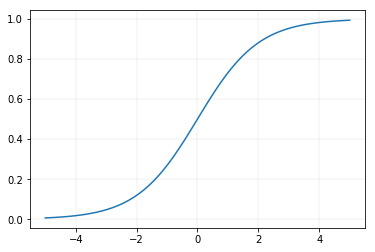
\includegraphics[width=.5\textwidth]{images/sigmoid.png}
\caption{Curva Sigmoidal}
\label{fig:sigmoid}
\end{figure}

Aplicando essa função no output de uma transformação linear, teremos como resultado um valor entre 0 e 1.

Além de a função sigmoide ser utilizada na estrutura de células de longa memória de curto termo (\textit{long-short term memory}) e células recorrentes bloqueadas (\textit{gated recurrent units}), também pode ser usada na saída do modelo. Poderíamos por exemplo, na classificação de sentimentos em texto, considerar valores próximos de 0 um sentimento negativo, e próximos de 1, positivo. Os valores maiores iguais a 0.5 serão classificados como positivos, enquanto 0.5 serão classificados como negativos.

\subsubsection{Tangente Hiperbólica}

Dada pela formula: 

\begin{equation}
    \sigma(Z) = 1/(1+e^{-Z})
\end{equation}

A imagem abaixo descreve a curva da tangente hiperbolica em um intervalo de 5 a -5.

\begin{figure}[!htb]
\centering
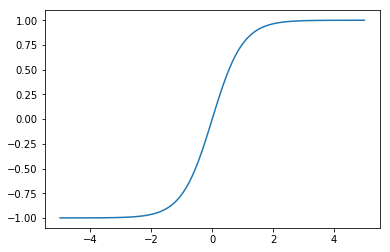
\includegraphics[width=.5\textwidth]{images/tanh.png}
\caption{Curva Tangente Hiperbólica}
\label{fig:tanh}
\end{figure}

Produz um resultado entre 1 e -1, e é usada na estrutura de células simples de redes recorrentes, células de longa memória de curto termo (\textit{long-short term memory}) e células recorrentes bloqueadas (\textit{gated recurrent units}). Em comparação a função de ativação sigmoide, possui a vantagem de ser simétrica em relação ao eixo x.

\subsection{Algoritmos de treinamento/Otimizadores}

\subsubsection{Escolha do Algoritmo de Otimização}

Infelizmente ainda não existe um consenso sobre qual é o melhor algoritmo de otimização. \cite{DBLP:journals/corr/SchaulAS13} apresentou uma comparação valiosa com um grande número de algoritmos de otimização através de uma ampla variedade de tarefas. Enquanto os resultados sugeriam que a família de algoritmos com taxa de aprendizado adaptativa (como RMSProp e AdaDelta \cite{DBLP:journals/corr/abs-1212-5701}) apresentavam na maioria das tarefas desempenho superior aos outros métodos, porém, não houve um único algoritmo que emergiu sobre os outros.

Atualmente, os algoritmos de otimização mais utilizados na literatura são Gradiente Descendente Estocástico, Gradiente Descendente Estocástico com Momento, RMSProp, RMSProp com Momento, AdaDelta \cite{DBLP:journals/corr/Ruder16} e Adam \cite{DBLP:journals/corr/KingmaB14}. A escolha de qual algoritmo de otimização usar, parece depender mais na familiaridade do desenvolvedor com o com o algoritmo (para afinar os hiperparametros mais facilmente) \cite{Goodfellow-et-al-2016}.

\subsubsection{Otimizador Adam}

Com a utilização do método \textit{minibatches}, cujo divide a base de dados em varios blocos chamados \textit{minibatches}, o progresso no gradiente tende a oscilar, logo o aprendizado pela rede se torna lento. Várias soluções foram propostas para solucionar esse problema, e a mais eficaz é uma junção das anteriores. O otimizador Adam \cite{DBLP:journals/corr/KingmaB14} utiliza a estimação do primeiro e do segundo momento dos gradientes, e terá a função de otimizar a função de custo.

\subsection{Função de Custo}

Um aspecto importante no desenvolvimento de redes neurais profundas é na escolha de função de custo. \cite{Goodfellow-et-al-2016}. As funções de custo de maneira geral são mecanismos para calcular a diferença entre os resultados do modelo, e os resultados desejados.

A escolha da função de custo foi baseada nos resultados alcançados no artigo de \cite{golik:2013}, onde são aplicadas e comparadas funções de custo em modelos de classificação, como reconhecimento de fala e reconhecimento de caracteres.

\subsubsection{Entropia Cruzada}

O cálculo do custo por entropia cruzada é dado pela seguinte formula:

\begin{equation}
    CE = -\sum\limits_{x} p(x)\log q(x)
\end{equation}

Onde $p(x)$ é o rótulo, e $q(x)$ o saída do modelo.
\subsection{Regularização}

Um problema central em aprendizado de máquina é como fazer um algoritmo que irá ter um bom desempenho não somente nos dados de treino, mas também em novos dados inseridos nele. Muitas estratégias usadas em aprendizado de máquina são explicitamente desenvolvidas para reduzir o erro no conjunto de teste, possivelmente à custa de um erro maior no conjunto de treino. Essas estratégias são conhecidas coletivamente como regularização \cite{Goodfellow-et-al-2016}.

O Dropout oferece pouco custo computacional, porém um método poderoso para regularização de uma ampla família de modelos \cite{DBLP:journals/corr/abs-1207-0580}.

Especificamente, dropout treina o conjunto consistindo através de sub-redes geradas pela remoção de unidades que fazem parte das camadas intermediarias ou de entrada, removendo uma proporção \textit{d} de neurônios temporariamente com base em um atributo \textit{p}, que indica a probabilidade. A remoção de neurônios pode desbalancear o aprendizado, logo o mesmo é normalizado para a quantidade de neurônios remanescente. A figura abaixo ilustra a técnica de dropout: \cite{Goodfellow-et-al-2016}.

\begin{figure}[!htb]
\centering
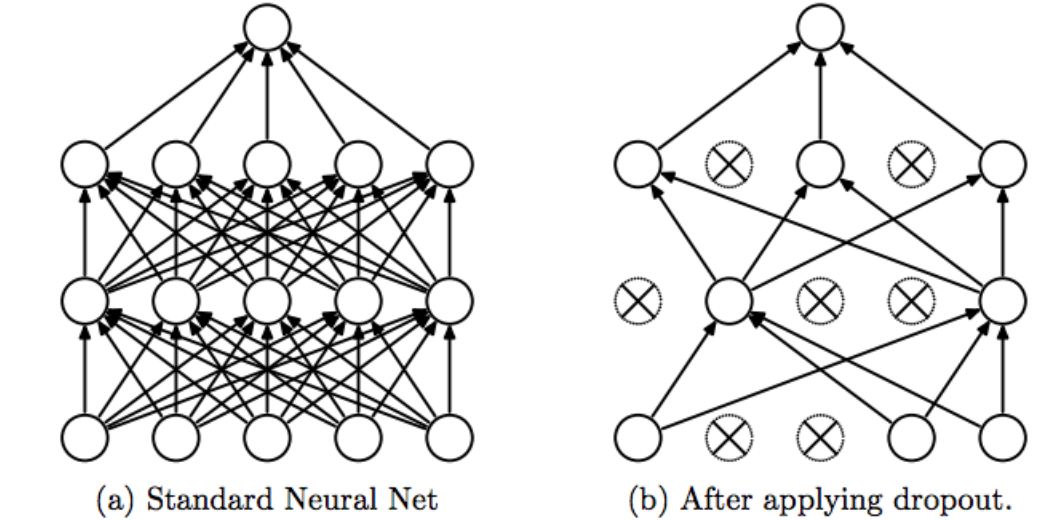
\includegraphics[width=.8\textwidth]{images/dropout.png}
\caption{Dropout}
\label{fig:dropout}
\end{figure}

\subsection{Inicialização de parâmetros}

Talvez a única propriedade conhecida com completa certeza é que parâmetros precisam de um início aleatório entre as diferentes unidades. Se duas unidades internas com a mesma função de ativação, estão conectadas às mesmas entradas, então essas unidades devem ter diferentes parâmetros iniciais. Caso elas tenham os mesmos parâmetros iniciais então um algoritmo de aprendizado determinístico aplicado à um modelo e função de custo também determinísticos, irá conseguintemente atualizar essas duas unidades da mesma forma. Mesmo se o modelo ou o algoritmo de treino for capaz de usar aleatoriedade para computar diferentes atualizações para diferentes unidades (por exemplo, dropout), na maioria das vezes é melhor inicializar cada unidade para computar uma função diferente de todas as outras unidades. Isso pode ajudar a garantir que nenhum padrão de entrada seja perdido no espaço nulo da forward propagation e nenhum padrão de gradiente seja perdido no espaço nulo da back-propagation. O objetivo de ter cada unidade computando uma funçao diferente motiva a inicialização aleatória de parâmetros \cite{Goodfellow-et-al-2016}.

Comumente, estabelecemos constantes os valores dos biases escolhidos de maneira heurística, e inicializamos apenas os pesos aleatoriamente (Goodfellow et al. 2017).

\subsection{Word Embeddings}

Word embedding é o nome coletivo de um conjunto de técnicas de modelagem de linguagem e de aprendizado de recursos no processamento de linguagem natural, em que palavras ou frases do vocabulário são mapeadas para vetores de números reais. Com base na proximidade entre palavras é possível codificar-las em um conjunto de parâmetros que definam aproximadamente seu significado. Nesse espaço de palavras, é possível realizar operações, sendo que cada dimensão indica alguma característica pertencente a determinado elemento. A figura 5 ilustra como funcionam esses vetores.
\begin{figure}
  \centering
  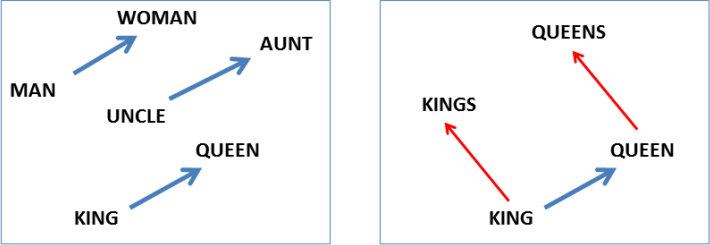
\includegraphics[width=1\textwidth]{images/wordembeddings.png}
  \caption{
    Representação de word embeddings. [Mikolov et al., NAACL HLT, 2013]
  }
  \label{}
\end{figure}

\subsubsection{Células recorrentes bloqueadas (GRU)}

Células normais de redes recorrentes não conseguem absorver grande as principais características de sentenças e sofrem de problemas como o desaparecimento do gradiente, durante o treino. As células recorrentes bloqueadas (\textit{gated recurrent units}) apresentam uma solução para esse problema.

São definidas pelas seguintes formulas:

\begin{equation}
    Ç<t> = tanh(Wc[\Gamma_r * c<t-1>, x<t>]+b_c)
\end{equation}

A equação (8) se refere ao cálculo do valor de ativação que será inserido na próxima célula recorrente bloqueada.

\begin{equation}
    \Gamma_u = \sigma(W_u[c<t-1>, x<t>]+b_u)
\end{equation}

A equação (9) se refere ao \textit{gate}, que dá nome a célula. É utilizado o valor da ativação da célula recorrente anterior e aplicada a função de ativação sigmoide, já detalhada na seção 3.3.2. A função sigmoide pode assumir apenas valores entre 0 e 1, sendo extremamente sensível aos valores de entrada. Logo essa operação tende a retornar valores ou muito próximos de 0 ou muito próximos de 1. Os resultados dirão quais elementos de \textit{c} serão atualizados por \textit{Ç}, ou seja, a saída de uma célula para outra, será apenas atualizada nos valores definidos por \Gamma_u.

Essa característica da célula recorrente bloqueada permite a memorização de características da sentença, como por exemplo, plural, gênero contexto, etc...

\begin{equation}
    \Gamma_r = \sigma(W_r[c<t-1>, x<t>]+b_r)
\end{equation}

A equação (10) se refere ao \textit{gate}, que define a relevância de \textit{c} na formação da ativação substituta \textit{Ç}.

\begin{equation}
    c<t>=\Gamma_u*Ç<t>+(1-\Gamma_u)*c<t-1)
\end{equation}

A equação (11) define a equação completa da célula recorrente bloqueada. É possível visualizar graficamente as equações descritas anteriormente através da figura (7).

\begin{figure}[!htb]
\centering
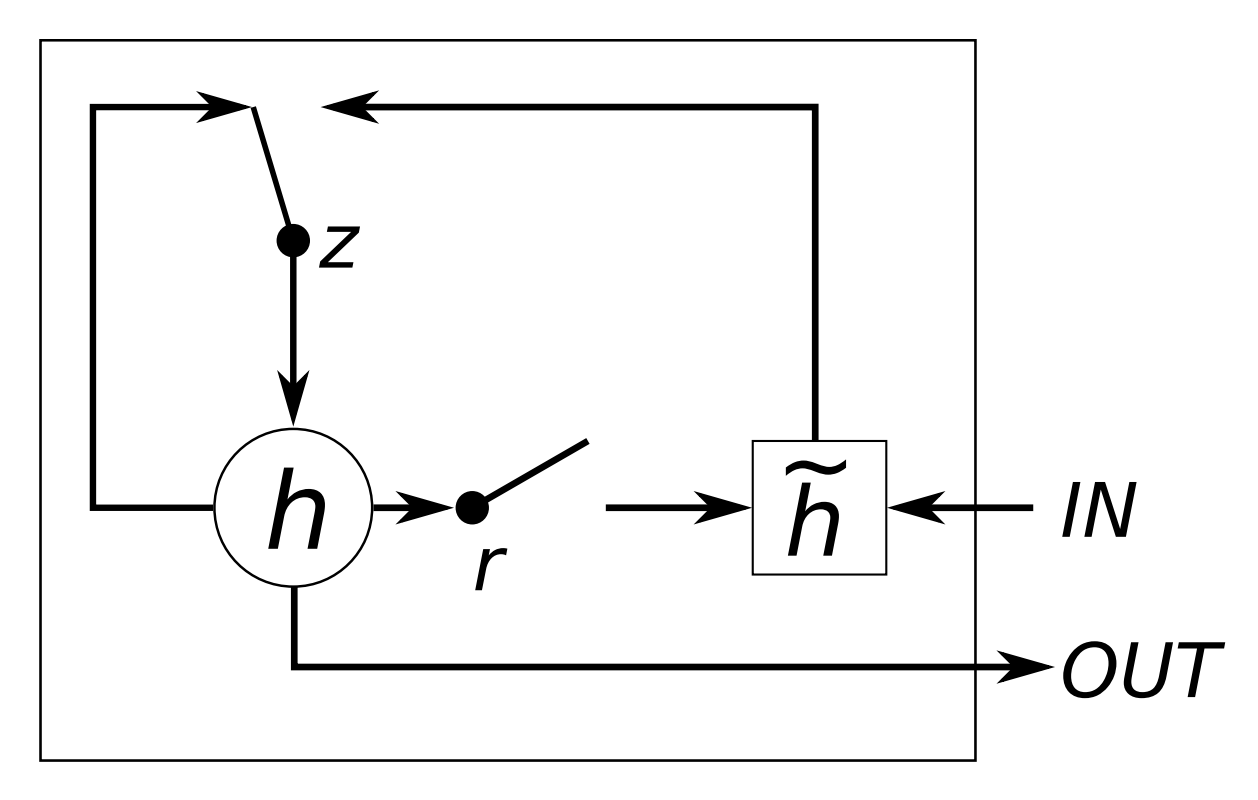
\includegraphics[width=0.4\textwidth]{images/gru_gate.png}
\caption{Esquema representativo da célula recorrente bloqueada \cite{DBLP:journals/corr/ChungGCB14}}
\label{fig:gru_gaet}
\end{figure}

\subsubsection{Longa memória de curto termo (LSTM)}

células de longa memória de curto termo (\textit{long-short term memory}) são definidas pelas seguintes formulas:

\begin{equation}
    Ç<t> = tanh(Wc[a<t-1>, x<t>]+b_c)
\end{equation}

A equação (12) é semelhante a equação (8) da célula recorrente bloqueada, porém não há o \textit{gate} referente a relevância da ativação anterior.

\begin{equation}
    \Gamma_u = \sigma(W_u[c<t-1>, x<t>]+b_u)
\end{equation}

A equação (13) representa o \textit{gate} que será utilizado para limitar a ativação \textit{Ç} na equação (16). É responsável por selecionar características da célula atual.

\begin{equation}
    \Gamma_f = \sigma(W_f[c<t-1>, x<t>]+b_f)
\end{equation}

A equação (14) representa o \textit{gate} que será utilizado para limitar a ativação \textit{c(t-1)} na equação (16).

É responsável por selecionar características da célula anterior.

\begin{equation}
    \Gamma_o = \sigma(W_o[c<t-1>, x<t>]+b_o)
\end{equation}

A equação (15) representa o \textit{gate} que será utilizado para limitar a ativação \textit{Ç} na equação (17).

É responsável por limitar a ativação final.

\begin{equation}
    c<t>=\Gamma_u*Ç<t>+(\Gamma_f)*c<t-1)
\end{equation}

\begin{equation}
    a<t>=\Gamma_o*c<t>
\end{equation}

A equação (17) define a equação completa da célula recorrente bloqueada. É possível visualizar graficamente as equações descritas anteriormente através da figura (8).

\begin{figure}[!htb]
\centering
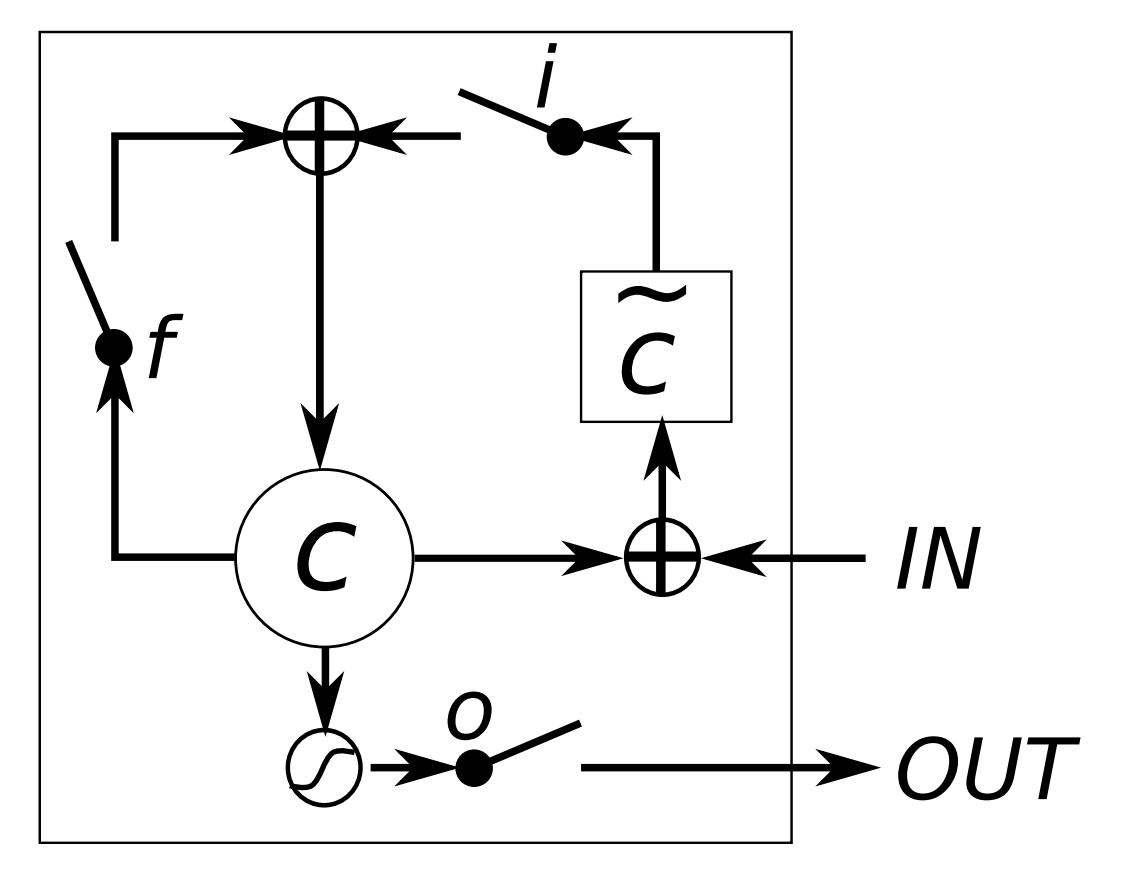
\includegraphics[width=0.4\textwidth]{images/lstm_gate.png}
\caption{Esquema representativo da célula de longa memória de curto termo \cite{DBLP:journals/corr/ChungGCB14}}
\label{fig:lstm_date}
\end{figure}

\subsection{Bidirecionalidade}
    A bidirecionalidade em redes neurais recorrentes, é um conceito ao qual a adição de elementos é feito duas vezes por sentença, a primeira vez em ordem normal e a segunda em ordem contrária (descrito pelo autor de forma positiva e negativa). Com esse conceito é removida a limitação de prever apenas a janela futura. A principal contribuição da bidirecionalidade, é adquirir o contexto de palavras no início da sentença. \cite{schuster1997bidirectional}.

\section{Arquiteturas Propostas}

Um modelo inicial foi definido rapidamente para obter o primeiro resultado, a seguir utilizamos a técnica de iteração. A técnica de iteração, consiste na ideia de definir uma arquitetura inicial, e definir hiperparâmetros rapidamente. Como ponto de partida, foi utilizado uma arquitetura bastante popular e extremamente efetiva, sendo sem transferência de aprendizado, o estado da arte.

\subsection{\textit{Word Embeddings}}

A matrix para representação de palavras indica os elementos de entrada de cada sentença, esse provém da técnica de Word Embeddings, detalhada na seção 3.7. Nesse trabalho foram utilizados vetores pré-treinados \textit{GloVe} \cite{pennington2014glove}, treinados em um \textit{crawler} com aproximadamente 840 bilhões de tokens.

\subsubsection{\texit{Pooling}}

Além de convoluções discretas, as operações de \textit{pooling} são outro importante bloco de construção nas CNNs. Operações de \textit{pooling} reduzem o tamanho de mapas de características (\textit{feature maps}) usando alguma função para resumir sub-regiões, como a média ou o valor máximo. O agrupamento funciona deslizando uma janela pela entrada e alimentando o conteúdo da janela para uma função de pooling. De certa forma, o pooling funciona como uma convolução discreta, mas substitui a combinação linear descrita pelo kernel com alguma outra função. A figura 9 fornece um exemplo de pooling máximo (\textit{max pool}).

\begin{figure}[!htb]
\centering
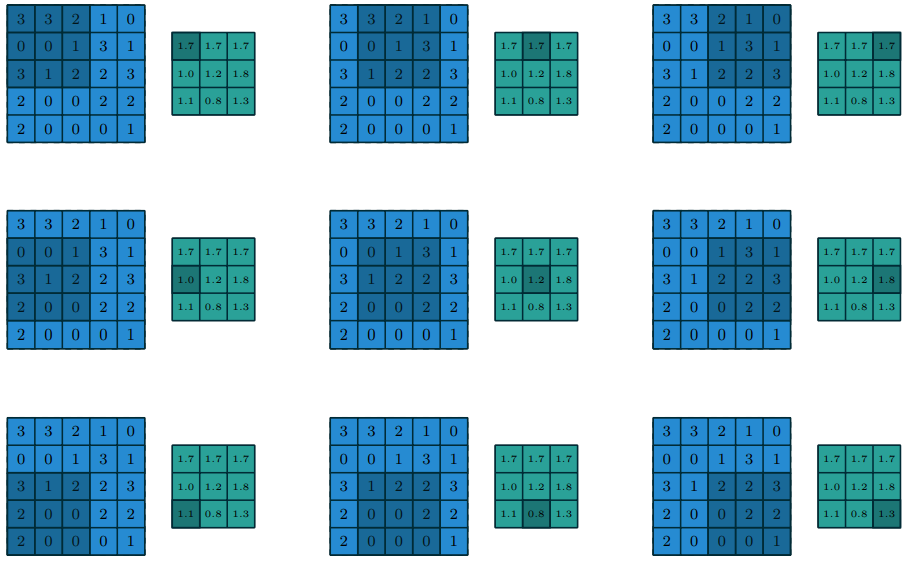
\includegraphics[width=.9\textwidth]{images/pooling.png}
\caption{Cálculo a saída de uma operação de pooling máximo. \cite{dumoulin2016guide}}
\label{fig:graph}
\end{figure}

\subsubsection{Célula}

As células utilizadas mudam o compartamento da rede neural recorrente, sendo que os casos utilizados nesse trabalho foram células recorrentes bloqueadas ou células de longa memória de curto termo, já definidas nas seções 3.7.1 e 3.7.2.

\subsubsection{Predição}

Predição faz uma rede neural totalmente conectada e utiliza a função de ativação sigmoide, já descrita na seção 3.3.2,  sendo que retornos maiores iguais a 0.5 serão considerados verdadeiros, e menores como falso.

\subsection{Rede recorrente}

Arquitetura base utilizada:

\begin{figure}[!htb]
\centering
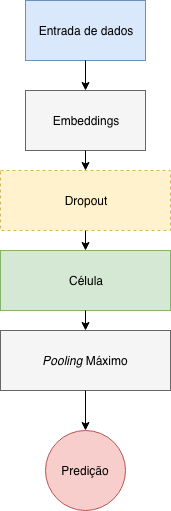
\includegraphics[width=.2\textwidth]{images/graph_2.png}
\caption{Rede recorrente simples}
\label{fig:graph_2}
\end{figure}

\subsection{Rede recorrente com convolução}

Arquitetura base utilizada:

\begin{figure}[!htb]
\centering
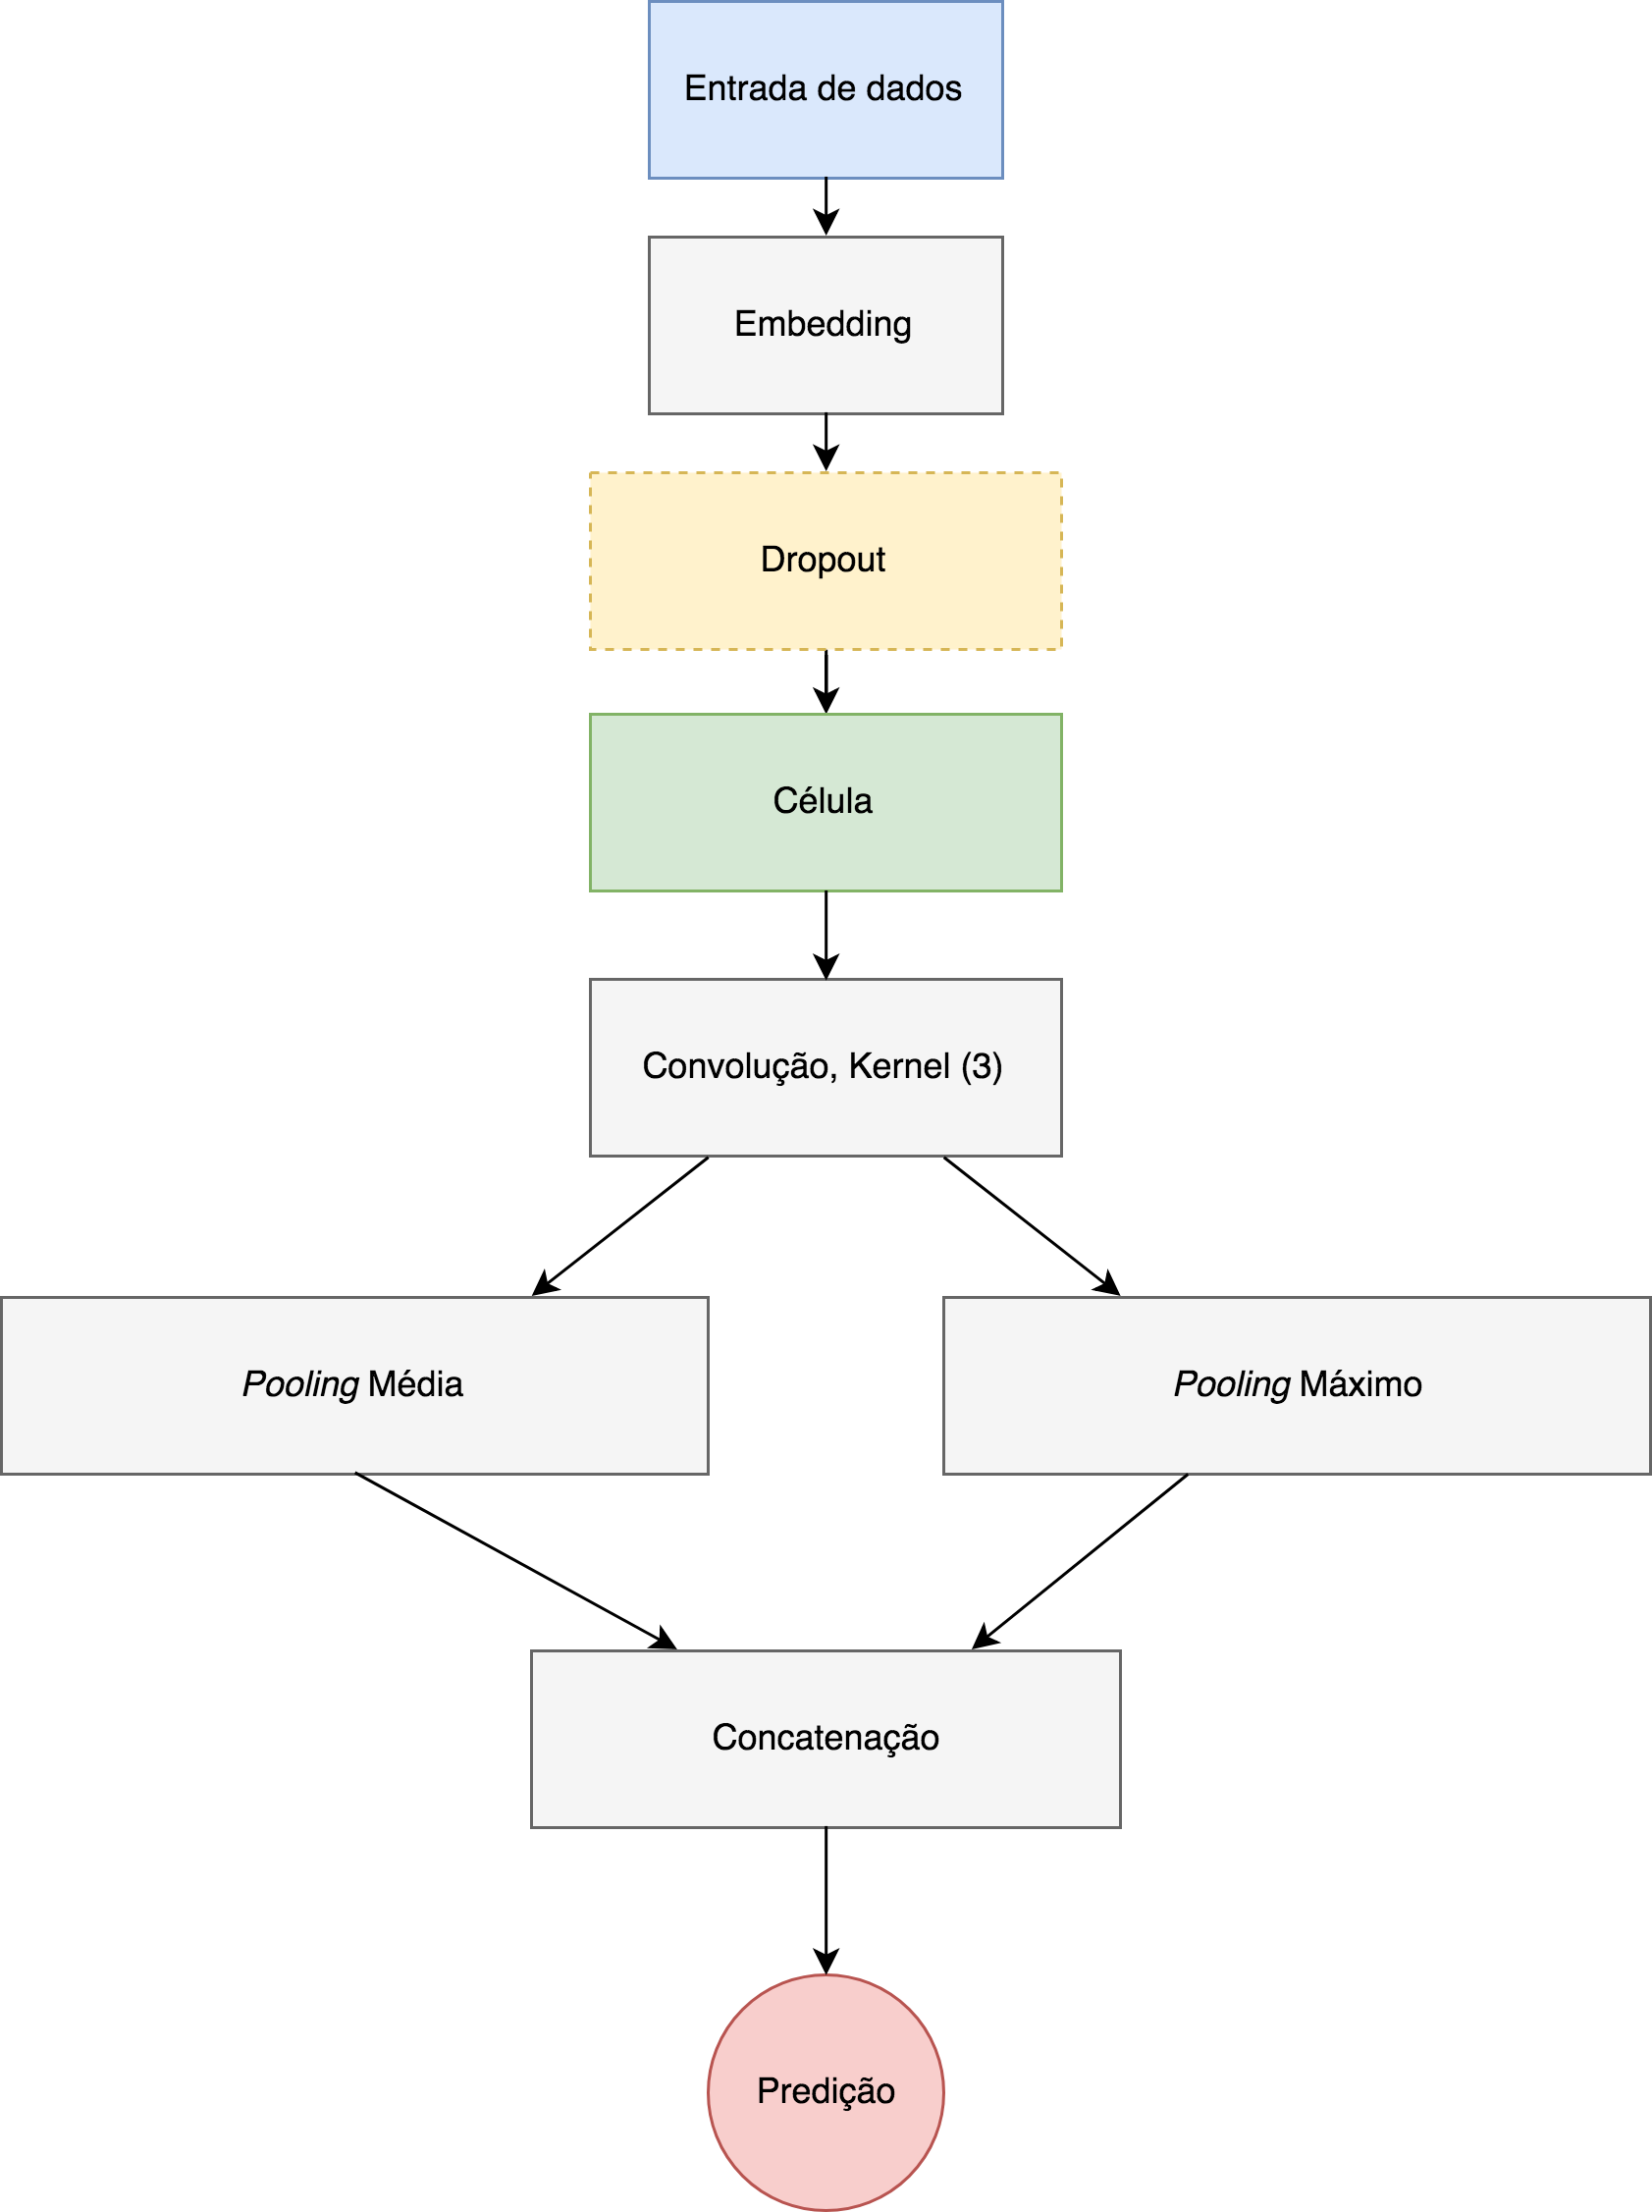
\includegraphics[width=.5\textwidth]{images/graph.png}
\caption{Rede recorrente com convolução.}
\label{fig:graph}
\end{figure}

\subsubsection{Convolução}

Uma convolução discreta é uma transformação linear que preserva uma noção de área. É esparso (apenas algumas unidades de entrada contribuem para uma determinada saída) e reutiliza parâmetros (os mesmos pesos são aplicados a vários locais na entrada). A Figura 11 fornece um exemplo de uma convolução discreta. A grade azul claro é chamada de mapa de recursos (\textit{feature map}) de entrada. Para manter o desenho simples, uma única entrada mapa de recursos é representado, mas não é incomum ter vários recursos mapas empilhados um sobre o outro.

Um kernel (área sombreada) de valor desliza pelo mapa de recursos de entrada. Em cada local, o produto entre cada elemento do kernel e o elemento de entrada que ele sobrepõe é computado e os resultados são somados para obter a saída na localização atual. o procedimento pode ser repetido usando kernels diferentes para formar o recurso de saída mapas conforme desejado. Os resultados finais deste procedimento são chamados mapas de recursos de saída. \cite{dumoulin2016guide}

\begin{figure}[!htb]
\centering
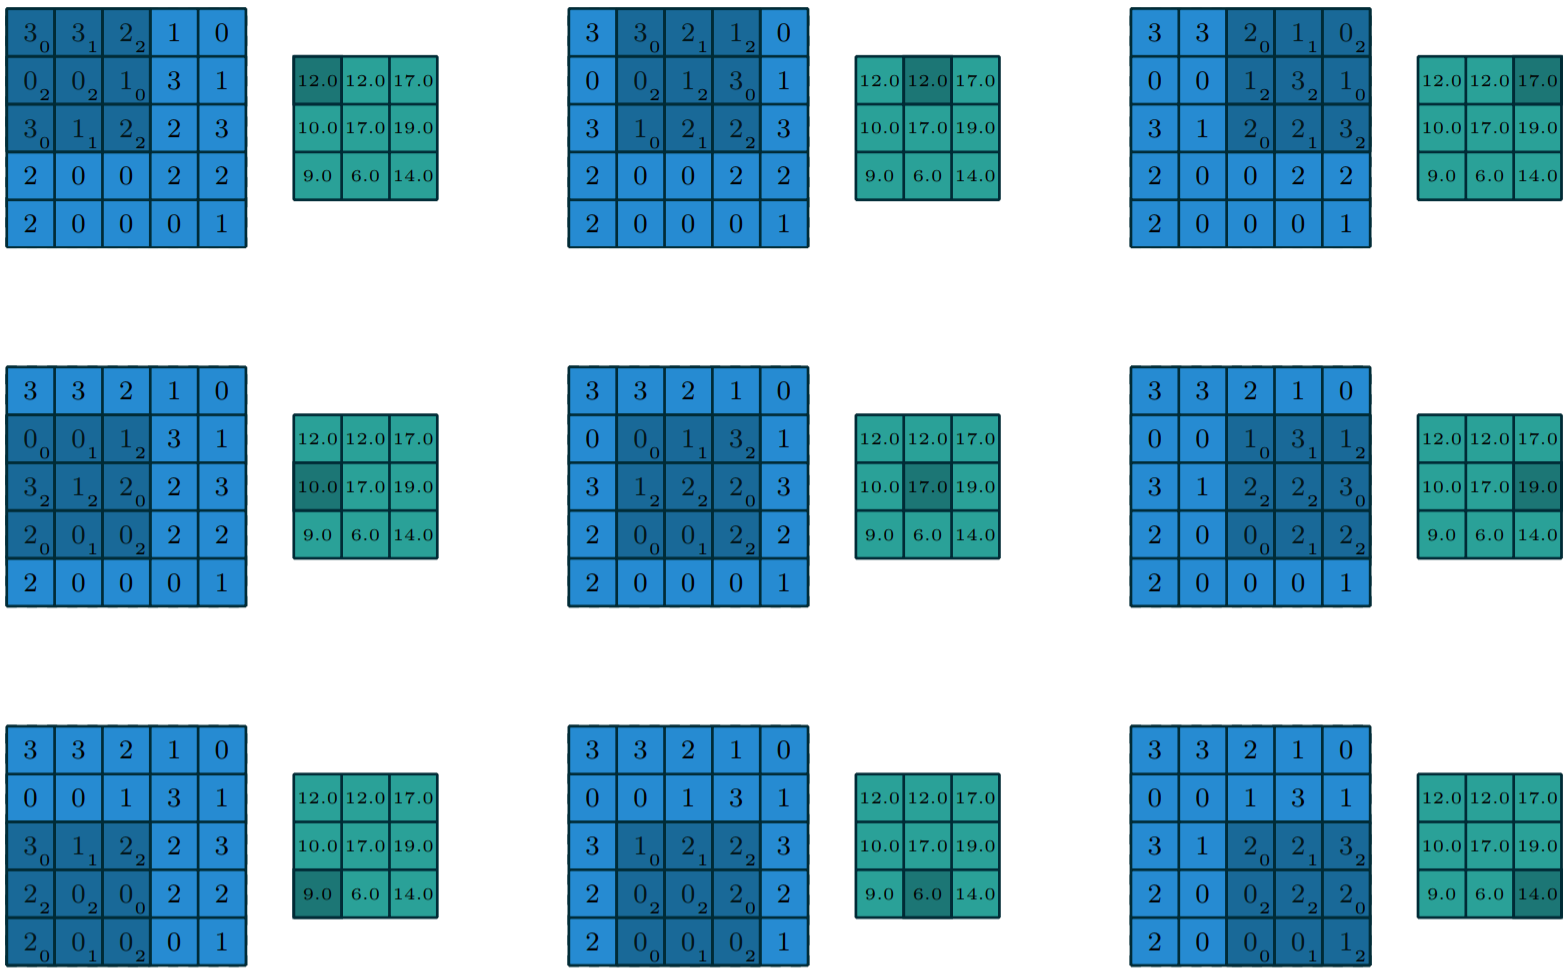
\includegraphics[width=.5\textwidth]{images/convolutions.png}
\caption{Cálculo a saída de uma operação de convolução. \cite{dumoulin2016guide}}
\label{fig:graph}
\end{figure}

\subsection{Hiper-parâmetros}

Embora a arquitetura do modelo contenha grande parte da informação sobre nossos modelos (seção 4.2 e 4.3), ainda é necessário definir alguns hiper-parâmetros que farão o comportamento de treino e arquitetura de nossa rede recorrente.

\begin{itemize}
  \item Durante a formação de matriz de \textit{embeddings} é possível definir a quantidade de parâmetros que cada palavra armazenará, foi escolhida de maneira arbitrária o valor de 300, que é compatível com matrizes já treinadas como por exemplo o \textit{GloVe} \cite{pennington2014glove}\\
  \item O número de nós na rede recorrente não possui uma métrica de escolha, foi escolhido com base no método iterativo, o valor de 256 nós.\\
  \item Regularização: Para evitar sobreajuste foi utilizada a técnica de \textit{dropout} com probabilidade \textit{p} de remover um nó de 0.5.\\
  \item O tamanho do \textit{minibatch} escolhido foi 128, esse valor se restringe ao tamanho da memória da placa gráfica utilizada para treino. Logo esse valor provou-se ideal em nosso hardware.\\
  \item O número de épocas escolhido para treinamento foi cinco, devido a limitação de hardware e quantidade de modelos a serem treinados, esse número demonstrou-se suficiente para garantir a convergência do modelo e evitar o ajuste exagerado, garantindo generalização.\\
  \item A taxa de aprendizado durante cada adição do gradiente por \textit{minibatch} foi escolhida arbitrariamente e de maneira iterativa, obtendo-seo valor de 1e-3.
\end{itemize}

Os hiperparâmetros do otimizador foram definidos através dos valores padrões indicados \cite{DBLP:journals/corr/KingmaB14}. A taxa de aprendizado utiliza do processo de iteração, e o valor utilizado nas análises preliminares é arbitrário, sendo inicialmente 1x10-3. Os pesos das células foram inicializador através da inicialização Glorot \cite{glorot:10}).

\subsection{Organização dos dados}

O banco de dados utilizou da técnica de separação de treino e teste, onde 90\% dos dados foi atribuída para treino e 10\% para validação. Não existe uma métrica fixa para a definição da quantidade a ser repartida, porém essa deve ser feita de acordo com a quantidade de dados rotulados. Como a validação segue apenas para verificar se não está acontecendo sobreajuste aos dados de treinamento, foi escolhido 10\% como dos hiperparametros. Essa técnica é conhecida como holdout. Em abordagens clássicas de aprendizado de máquina, normalmente é utilizada a validação cruzada, porém, em casos de aprendizagem profunda (\textit{deep learning}) isso se torna inviável devido a quantidade de processamento, já que nesse tipo de validação é necessário treinar o modelo \textit{k} vezes, onde \textit{k} é um hiperparâmetro. Como modelos de aprendizagem profunda (\textit{deep learning}) possuem grande volume de dados, utilizaremos o holdout devido a viabilidade computacional.

A segmentação a seguir representa como os dados foram separados:

\begin{figure}[!htb]
\centering
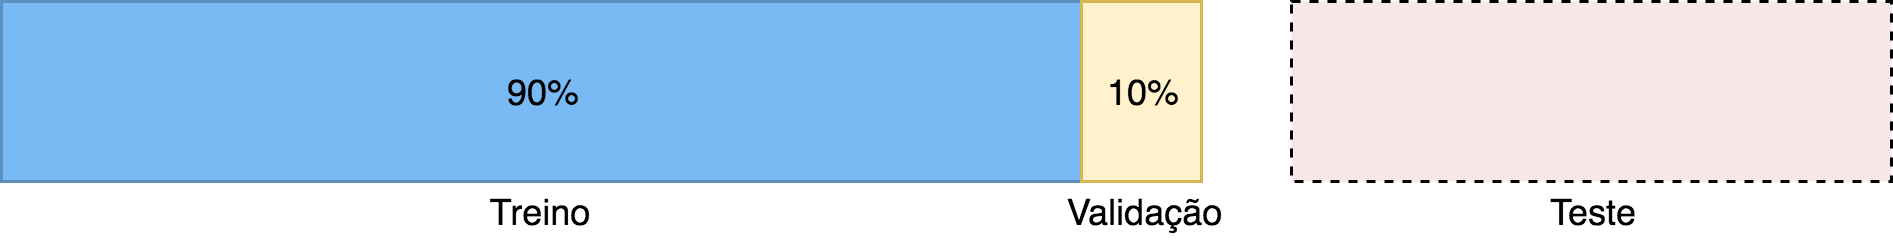
\includegraphics[width=1\textwidth]{images/datasplit.png}
\caption{Separacão de dados}
\label{fig:datasplit}
\end{figure}

A segmentação de testes não está inclusa nos dados públicos. Tal teste é feita através de dados não rotulados na plataforma Kaggle. É possível realizar um submissão com os rotulos e obter a acurácia. Essa segmentação não é de acesso público para evitar que modelos sobreajustem seus parâmetros, assim o resultado retornado garante a validade de generalização do modelo.

\section{Análises de resultados}

Em primeira instância os modelos obtiveram resultados satisfatórios, alcançando acurácia próxima à melhor submissão deste problema.

\begin{table}[!htb]
  \small
  \centering
  \renewcommand{\arraystretch}{1.15}
  \begin{tabular}{llll}
      \hline
      \multicolumn{4}{c}{Modelo monolítico, treinado por 5 épocas} \\
      \hline
    \hline
     Célula & Acurácia Treino & Acurácia Validação & Acurácia Teste \\
    RNN & 97,99\% & 98,19\% & 97,38\% \\
    GRU & 98,32\% & 98,35\% & 98,09\% \\
    LSTM & 98,29\% & 98,41\% & 98,12\% \\
    GRU Bidirecional & 98,37\% & 98,38\% & 98,15\% \\
    LSTM Bidirecional & 98,37\% & 98,40\% & 98,22\% \\
    GRU + Convolução & 98,37\% & 98,31\% & 98,22\% \\
    LSTM + Convolução & 98,35\% & 98,42\% & \textbf{98,25}\% \\
    GRU Bidirecional + Convolução & \textbf{98,41}\% & 98,44\% & 98,18\% \\
    LSTM Bidirecional + Convolução & \textbf{98,41}\% & \textbf{98,48}\% & 98,15\% \\
    \hline
  \end{tabular}
  \caption{Resultados}
  \label{tab:ptb}
\end{table}


Podemos observar que nesse conjunto de dados a bidirecionalidade não trás beneficios nestas instâncias. A convolução trouxe ganhos em todos os casos sem bidirecionalidade. Ainda é possível analisar que os modelos bidirecionais e com convolução tiveram os melhores resultados no treino e validação, porém não se generalizaram no caso de teste, tal situação demonstra sobreajuste por parte desses modelos nos dados de treino e validação.

Análises utilizando modelos de linguagem e transferência de aprendizado ainda estão sendo desenvolvidas.

O repositório com códigos fontes de todos os modelos analisados está disponível no Github, através do endereço: \url{https://github.com/pstwh/toxic-comments-keras}. É recomendado a utilização de placa gráfica para reprodução desses artigos. As configurações utilizadas pelos autores para treinamento e validação dos modelos: Placa gráfica NVIDIA Quadro M4000, 30 Gb memória RAM e processador Intel® Xeon® E5-2623 v4 8 núcleos.

\section{Considerações Finais e Trabalhos Futuros}

Nesse trabalho apresentamos métodos automátizados para análise de comentários tóxicos utilizando redes recorrentes e suas variações. O conjunto de dados utilizado foi adquirido da plataforma \textit{Kaggle}, onde foram tratados e processados com a utilização de \textit{word embeddings} provenientes da \textit{GloVe} \cite{pennington2014glove}.

A comparação dos modelos testados demonstra como a combinação de modelos recorrentes e camadas convolucionais melhoram a acurácia. Técnicas como transferência de aprendizado em modelos de linguagem não foram aplicadas nesse trabalho, porém há ambição de aplica-los em trabalhos futuros. Há a possibilidade de reelaborar a célula que constrói a rede neural recorrente para atender melhor a este caso. Talvez a aplicação de uma rede de capsulas \cite{DBLP:journals/corr/abs-1710-09829} proporcionaria um resultado superior devido a não variação em translações, que é uma das características desta arquitetura.

Existe a ambição em trabalhos futuros de aplicar conceitos presentes nesse artigo em outros conjuntos de dados, como por exemplo conjuntos de dados em português do brasil, com ajuda de aprendizagem semi-supervisionada e transferência de aprendizado.

\bibliographystyle{templates/sbc}
\bibliography{bibliography}

\end{document}
